\begin{figure*}[h]                                                           
 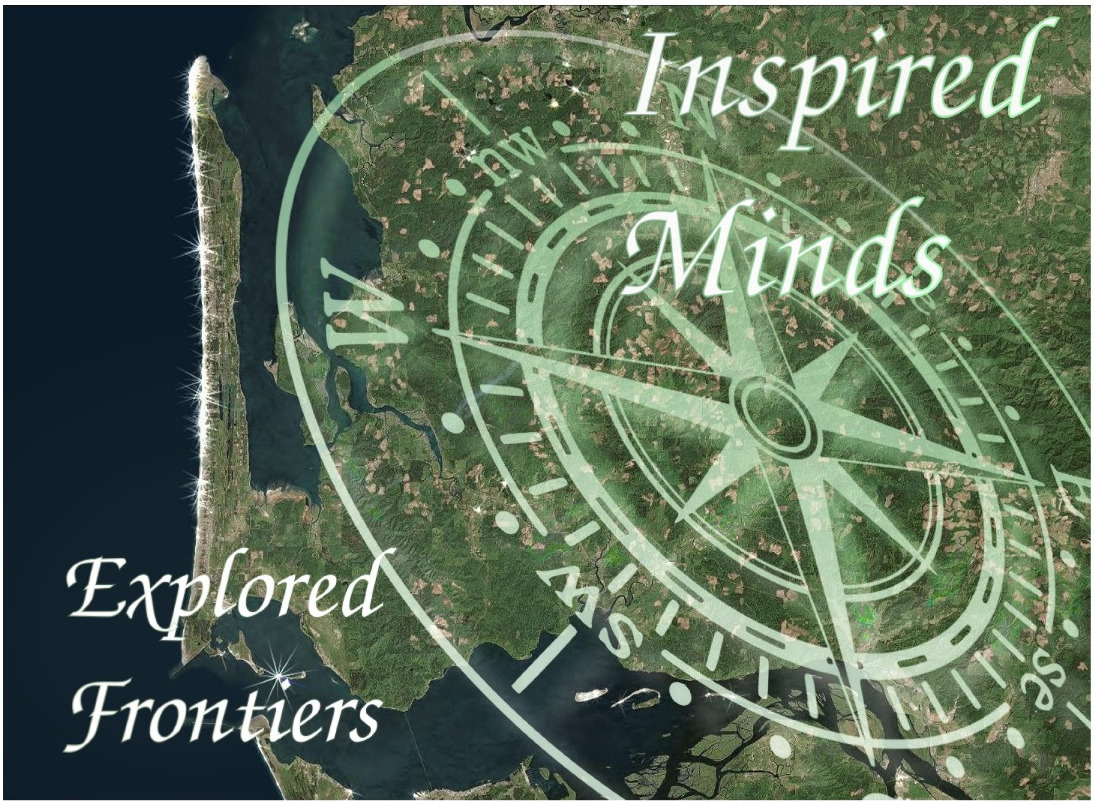
\includegraphics[width=\linewidth]{./media/images/engaged}%
  \small{\textsc{\\ Imagine your readers' feeling} knowing they tackled mind and matter to complete the Quest (Photo:
    \href{http:portfolio.cooper.stevenson.name}{\textsc{D. Cooper Stevenson).}}}
  \label{fig:engaged}%                                                 
\end{figure*}                                                                
\begin{quotation} 
\noindent\color{Sepia}{\scriptsize{\textit{\textbf{“Ease of navigation is important in both physical and virtual space.” }}}}\\[2mm]
   \hfill\color{Sepia}{\scriptsize{\textendash John Quelch}}
\end{quotation} 

\section{updates and expansion}
This edition of \textit{Discoverer's Digest} is necessarily a rolling release
edition of the magazine. As Voltaire quotes the Itallian proverb, ``Don’t let
the perfect be the enemy of the good.'' In the next week or so I will update
these articles with the specific code samples necessary to create the plots,
etc. I described in the article. I feel this especially important as
\href{http://ifcomp.org}{\textsc{ifcomp}} is hot underway; should I give just
one author a spark of inspiration to improve his entry I will have considered
this work a sucess.

\subsection{upcoming issue}
In the next issue of \textit{Discoverer's Digest} I tackle in concrete terms
extended areas of \textsc{if} that are sometimes discussed but not, at least as
far as I am aware, fully implemented.

First up brings the power of \textsc{tads} to hook the ``real world'' into your
work of \textsc{if}. Specifically I show an example and code for using
\textsc{gps} in your next adventure. For now I leave you with
\href{http://portfolio.cooper.stevenson.name/tarlatt/tarlatt_slough_trail_feature_demo.mp4}{\textsc{this
    partial walkthrough}} exploring a trail along Willapa Bay in Long Beach, WA.

Also, I'll build on the plotting I described in this issue to explore using
Natural Language Processing to make ``filling in the blanks'' of your work
faster, fuller, and comprehensive.

\subsection{``adieu'' \& additions}
Your sumissions of news, musings, or reviews/announcements of new works are
always welcome. Simply \href{mailto:cooper@cooper.stevenson.name}{\textsc{send
    me a personal email}} to submit.

Until next time (and as always), I wish you the best in your enjoyment of the
medium! \\ \\

\noindent Fair Winds, \\ \\

\noindent \href{mailto:cooper@cooper.stevenson.name}{\textsc{D. Cooper Stevenson}} 

